\documentclass[tikz, border = 1 cm]{standalone}
\usepackage{tikz}
\usepackage{tikz,bm}
\usetikzlibrary{shadows.blur}
\usetikzlibrary{angles,arrows,calc,quotes}
\usetikzlibrary{patterns}
\usetikzlibrary{shapes}

\usetikzlibrary{%
    decorations.pathreplacing,%
    decorations.pathmorphing,%
    calc,%
}

\usetikzlibrary{calc,fadings,decorations.pathreplacing,arrows,positioning}

\usepackage{tkz-euclide}

\begin{document}
    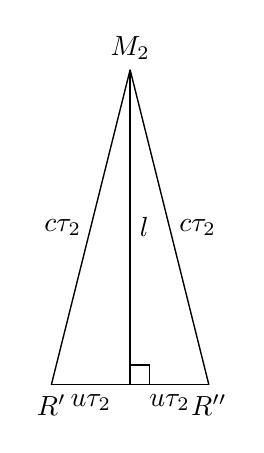
\begin{tikzpicture}
      \newcommand{\angledroit}[1][2]
                 {\draw[#1] (0,0.25)-|(0.25,0);
                 }
                 

      \draw[line width=.5pt](-1,0) -- (1,0);
      \draw[line width=.5pt](0,0) -- (0,4);
      \draw[line width=.5pt](-1,0) -- (0,4);
      \draw[line width=.5pt](1,0) -- (0,4);
      \angledroit[shift={(0,0)}];

      \node[below] at (-1,0) {$R'$};
      \node[below] at (1,0) {$R''$};
      \node[below] at (-0.5,0) {$u\tau_2$};
      \node[below] at (0.5,0) {$u\tau_2$};
      
      \node[left] at (-0.5,2) {$c\tau_2$};
      \node[right] at (0.5,2) {$c\tau_2$};

      \node[right] at (0,2) {$l$};

      \node[above] at (0,4) {$M_2$};
    \end{tikzpicture}
    \end{document}
